% kompilace xelatex prezentace.tex
% dokumentace k beameru: http://ftp.cvut.cz/tex-archive/macros/latex/contrib/beamer/doc/beameruserguide.pdf

% nastavení formátu prezentace 16:9
\documentclass[czech,aspectratio=169]{beamer}

\usepackage{polyglossia}
\setmainlanguage{czech}
\usepackage{ulem}
\usepackage{relsize}
\usepackage{xspace}
\newcommand{\Rplus}{\protect\hspace{-.1em}\protect\raisebox{.35ex}{\smaller{\smaller\textbf{+}}}}
\newcommand{\Cpp}{\mbox{C\Rplus\Rplus}\xspace}

% nastavení vzhledu
% další možnosti vzhledu viz https://hartwork.org/beamer-theme-matrix/
\usetheme{Boadilla}
\usecolortheme{dove}

% vzhled slajdů vnitřní téma (např. vzhled odrážek)
\useinnertheme{circles} %možnosti: default circles rectangles rounded inmargin
% vzhled slajdů vnější téma
\useoutertheme{default} %možnosti: default, miniframes, smoothbars, sidebar, split, shadow, tree, smoothtree, infolines

% zavedeme čvutí modou barvu
\definecolor{CVUT}{HTML}{0065BD}
% čvutí modou použijeme jako hlavní barvu prezentace
\setbeamercolor{structure}{bg=white,fg=CVUT}

% jako font prezentace nadefinujeme oficiální ČVUT písmo Technika
% https://www.cvut.cz/logo-a-graficky-manual  -- inforek, příhlášení přes celoškolské heslo
%\usepackage{fontspec}
%\setsansfont{Technika-Kniha}

% vypneme navigační panel beamer (pro zapnutí zakomentujeme)
\beamertemplatenavigationsymbolsempty{}

% vygenerujeme slajdy s poznámkami
%\setbeameroption{show notes}

% vygeneruje slajdy s poznámky vhodné pro promítání na dvou monitorech
%\usepackage{pgfpages}
%\setbeameroption{show notes on second screen}

% další balíčky
\usepackage[outputdir=build]{minted}
\usepackage{hyperref}

% Údaje o prezentaci
\title[Nástroj pro konfiguraci a monitorování]{Nástroj pro konfiguraci a monitorování}
\subtitle{Bakalářská práce}
\institute[FIT ČVUT v Praze]{Fakulta informačních technologií \\ České vysoké učení technické v Praze}
\author[V. Kubernát]{Václav Kubernát \\ Vedoucí práce: Ing. Tomáš Čejka, Ph.D.}
\date{20. 6. 2019}
\titlegraphic{
\includegraphics[width=.1\textwidth]{logo-cvut}}


\begin{document}


\begin{frame}
    \titlepage{}
\end{frame}

\begin{frame}{Motivace}
    \begin{itemize}[<+->]
        \item CESNET
        \item Czechlight
    \end{itemize}
\end{frame}

\begin{frame}{Konfigurace}
    \begin{itemize}
        \item Provozovaná zařízení je nutné konfigurovat\pause{}
        \item Standardizace konfigurace\pause{}
        \item NETCONF\pause{}
            \begin{itemize}
                \item klient-server
                \item komunikace pomocí XML
                \item modelovaní konfigurace pomocí schémat YANG
            \end{itemize}
    \end{itemize}
\end{frame}

\begin{frame}{Existující konfigurační nástroje}
Serverová část:
\begin{itemize}
    \item Netopeer2-server a sysrepo
\end{itemize}\pause{}
Klientská část:
\begin{itemize}
\item Netconf2-cli
\item sysrepocfg
\end{itemize}
\end{frame}

\begin{frame}[fragile]{Intuitivita}
    \begin{columns}
        \pause{}
        \begin{column}{.47\textwidth}
            \verb|$ ed|

            \pause{}
            \verb||

            \verb|?|

            \pause{}
            \verb|help|

            \pause{}
            \verb|?|

            \pause{}
            \verb|h|

            \pause{}
            \verb|Invalid address|

            \pause{}
            \verb|quit|

            \verb|?|

            \pause{}
            \verb|exit|

            \verb|?|
            \pause{}
        \end{column}
        \begin{column}{.47\textwidth}
            \verb|~/example$|\pause{} \verb|ls|

            \pause{}
            \verb|file1  file2  file3|

            \verb|~/example$|\pause{} \verb|echo Hello > file1|

            \verb|~/example$|\pause{} \verb|cat fi| \pause{}

            \verb|~/example$| \verb|cat file|
            \pause{}
            \verb|file1  file2  file3|

            \verb|~/example$ cat file|\pause{}\verb|1|
            \pause{}
            \verb|Hello|
        \end{column}
    \end{columns}
\end{frame}

\begin{frame}{Architektura}
    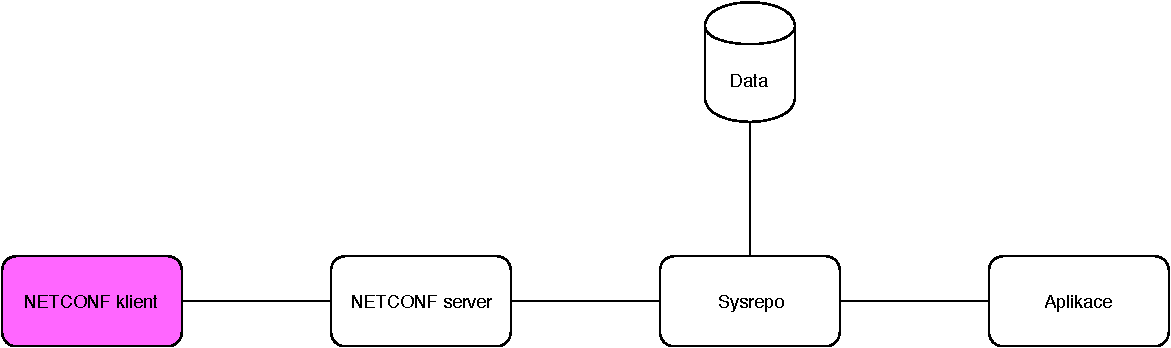
\includegraphics[width=.9\textwidth]{overview}
\end{frame}

\begin{frame}[plain,label=tokDat]
\begin{center}
    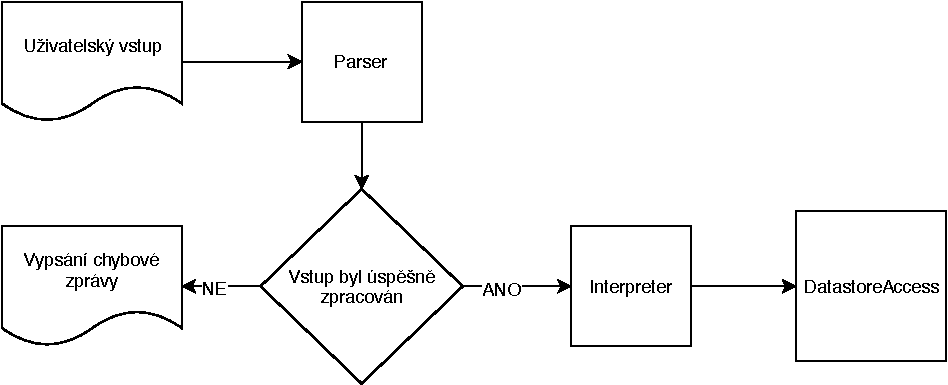
\includegraphics[width=.9\textwidth]{diagram}
\end{center}
\end{frame}

\begin{frame}{Parser}
    \begin{itemize}[<+->]
        \item Zpracovává uživatelský vstup
        \item Dynamický -- je vytvářen za běhu z konkrétních dat
        \item Abstraktní rozhraní Schema
            % říct konkrétní
        \item Generuje data pro automatické doplňování
    \end{itemize}
\end{frame}

\againframe<1>{tokDat}

\begin{frame}{Komunikace s datovými úložišti}
    Abstraktní rozhraní DatastoreAccess\pause{}
    \vfill
    Komunikace se sysrepo démonem\pause{}
    \begin{itemize}[<+->]
        \item urychlení vývoje
        \item zjednodušení aplikace -- NETCONF server není nutný
    \end{itemize}

    \vfill

    \only<-4>{\ }
    \only<5>{NETCONF rozhraní jako POC}
\end{frame}

\begin{frame}<1,2,3>[fragile,label=porovnani]{Porovnání s \textit{Netopeer2-cli}}
    Změna hodnoty example:leafInt na 5.
    \vfill
    \begin{columns}
        \pause{}
        \begin{column}{.47\textwidth}
            \verb¨// ... připojení k serveru ...¨

            \verb¨>¨\pause{} \verb|edit-config --target --config|

            \pause{}
            \verb¨OK¨

            \verb¨>¨\pause{} \verb|commit|

            \pause{}
            \verb¨OK¨

            \verb¨>¨

        \end{column}
        \pause{}
        \begin{column}{.47\textwidth}
            \verb¨// ... připojení k serveru ...¨

            \verb¨>¨\pause{} \verb|set |

            \pause{}
            \verb¨example:leafInt example:leafString¨

            \verb¨> set example:leaf¨\pause{}\verb|I|\pause{}\verb|nt|\pause{} \verb|5|

            \pause{}
            \verb¨>¨\pause{} \verb|commit|

            \verb¨>¨
        \end{column}
    \end{columns}
\end{frame}

\begin{frame}[plain,fragile]
    \verb¨    <!--#¨

    \verb¨    Type the content of the <edit-config>.¨

    \verb¨    -->¨

    \color{gray}
    \verb¨    ~¨

    \verb¨    ~¨

    \verb¨    ~¨

    \verb¨    ~¨

    \verb¨    ~¨

    \verb¨    ~¨

    \verb¨    ~¨

    \verb¨    ~¨

    \verb¨    ~¨

    \verb¨    ~¨

    \verb¨    ~¨

\end{frame}
\begin{frame}[plain,fragile]
    \verb¨    <leafInt xmlns="http://example.com">5</leafInt>¨

    \color{gray}
    \verb¨    ~¨

    \verb¨    ~¨

    \verb¨    ~¨

    \verb¨    ~¨

    \verb¨    ~¨

    \verb¨    ~¨

    \verb¨    ~¨

    \verb¨    ~¨

    \verb¨    ~¨

    \verb¨    ~¨

    \verb¨    ~¨

    \verb¨    ~¨

    \verb¨    ~¨

\end{frame}

\againframe<4->{porovnani}


\begin{frame}{Shrnutí}
    \begin{itemize}
        \item Identifikace nevýhod současných řešení
        \item Implementace aplikace, která problémy mitiguje
        \item Generičnost aplikace zajišťuje podporu i pro jiná zařízení
        \item Aplikace je již testována na reálných zařízeních
    \end{itemize}
\end{frame}
\end{document}
